\section{Hyperparameters}
In order to find the optimal hyperparameters,
multiple experiments are run,
exploring different hyperparameters.

The hyperparameters which are expected to be mostly independent from others are checked first.
Then, the remaining hyperparameters are checked in a grid search. %TODO: not yet

In each case, 10-fold cross-validation was utilized to reduce the variance of single data points.


\subsection{Batch size}
The \emph{batch size} determines the number of events used for each training step.
While larger batch sizes increase the speed of training
on optimized hardware,
the performance of the model can be negatively affected \cite{batchsize_kandel}.
% NOTE: not-so-relevant citation

% TODO: RUN THIS EXPERIMENT


\subsection{Adaptive step size: $J$-factor}
The adaptive step size function internally relies on clustering the data into $J$ clusters.
The number of clusters $J$ is therefore a hyperparameter of the algorithm.
Because of the dependence of …,
$J$ is not used directly.
Instead, the \emph{J-factor} is used,
which is defined as $J$ divided by the number of bins.

\begin{figure}
  \centering
  % TODO: correct dimensions
  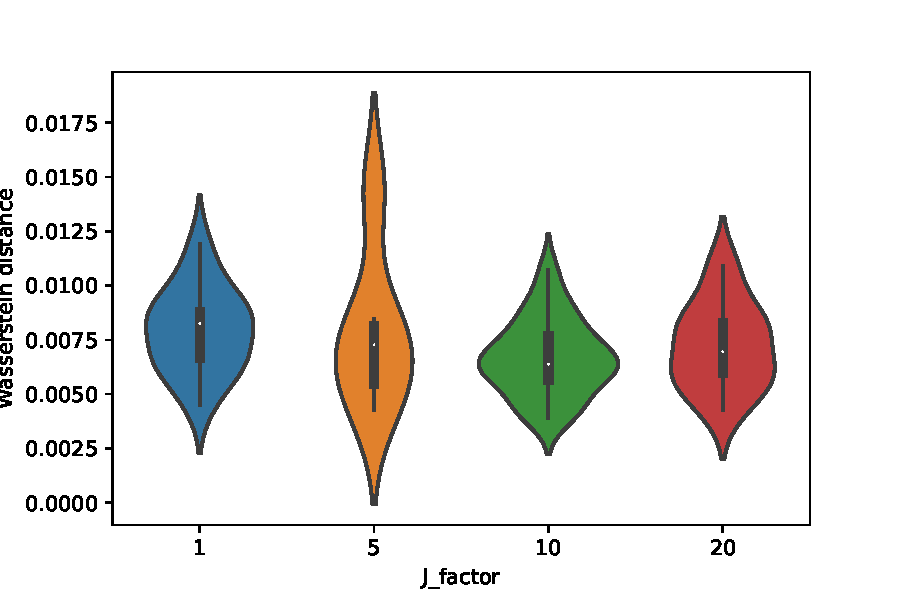
\includegraphics[scale=1]{content/plots/halftime/wd_per_J_factor.pdf}
  \caption{Violin plot of the Wasserstein distance for different $J$-factors.}
  \label{fig:hyperparameter:J_factor}
\end{figure}


\subsection{Number of epochs \& $\epsilon$}
While a higher number of epochs typically increases the model's performance on the training data,
it also increases the risk of overfitting.


When using adaptive step sizes,
instead of specifying a fixed number of DSEA iterations,
a minimum $\Chi^2$ distance between iterations $\epsilon$
can be specified.
When the $\Chi^2$ distance becomes smaller than $\epsilon$,
convergence is assumed and the training is stopped.
